Before starting to concept the graphical discuss system, it's necessary to analyse requirements and objectives behind the origin motivation in the first place. It should be defined at first, what kind of functionalities should be achieved and how the system behaves.

\subsection{Basic Functionalities}

As a graphical discuss system for the educational purpose, the system should contain basic functionalities on the prototype  of a forum which could be organized by classes. So class management, question management and answer management are the three essential parameters to be designed at the start.

\subsubsection{Course Management}

Each question should have a certain domain of its content, so the questions are organized by classes initially. The features of course management should be:

\begin{enumerate}
\item
\textbf{Create Course}: The user who is identified as a tutor is able to create course and maintain the course he created. While creating the course, the tutor can define the name of the course and upload an image as a background of the course for better recognization. In addition, concret description of the course could also be added to the description area.

\begin{figure}[!htbp]
  \caption{placeholder}
  \centering
    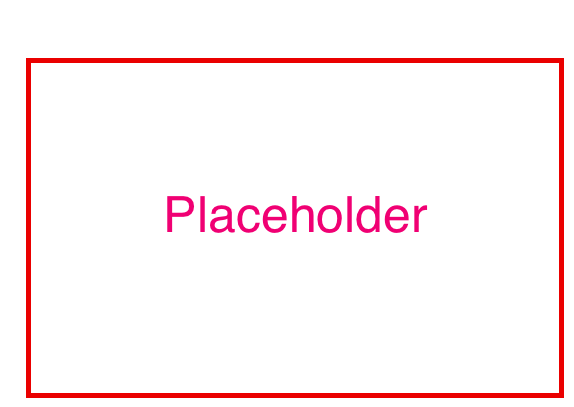
\includegraphics[width=0.6\textwidth]{Figures/placeholder.png}
  \label{fig:placeholder}
\end{figure}

% Mockups create, upload, description

\item
\textbf{Search Course}: After a course is created, a corresponding unique identifier code for the course will be generated at the same time. The students are able to find the course through the identifier code.

\begin{figure}[!htbp]
  \caption{placeholder}
  \centering
    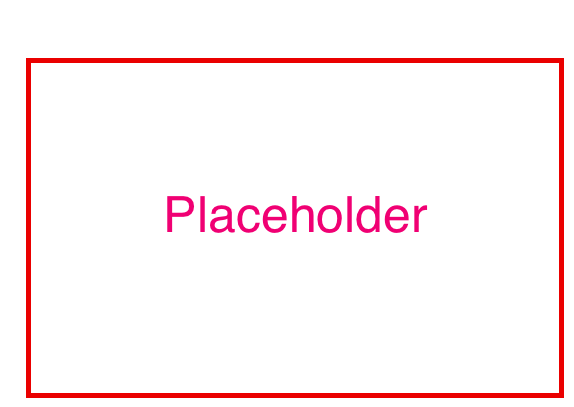
\includegraphics[width=0.6\textwidth]{Figures/placeholder.png}
  \label{fig:placeholder}
\end{figure}
% Mockups code, search

\item
\textbf{Favor Course}: If a student is interest to a certain course, he is capable to add the course to his favor list so that it's easy to find and access the course he liked later.

\begin{figure}[!htbp]
  \caption{placeholder}
  \centering
    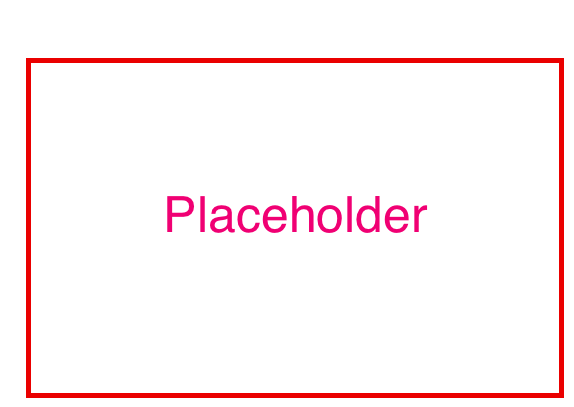
\includegraphics[width=0.6\textwidth]{Figures/placeholder.png}
  \label{fig:placeholder}
\end{figure}
% Mockups fav button, fav list.

\end{enumerate}

\subsubsection{Question Management}

\begin{enumerate}
\item
\textbf{Submit/Edit/Withdraw Question}: The student who has confusion with the teaching content can submit his own question with detailed description in a certain course. The user is also permitted to edit the question if he want to add more precise informations or modify the unclarity he made to the question. Withdrawing of his own question is also possible, but only when there're no contributes made to the question.

\begin{figure}[!htbp]
  \caption{placeholder}
  \centering
    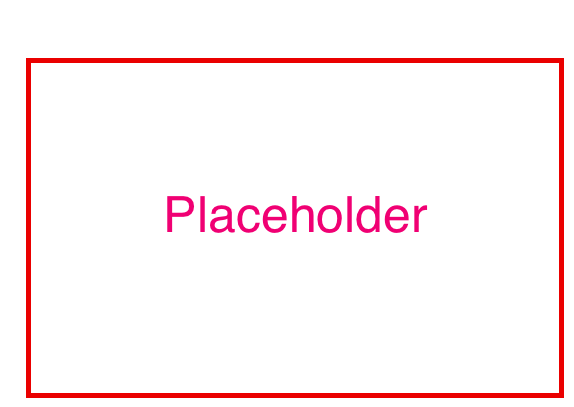
\includegraphics[width=0.6\textwidth]{Figures/placeholder.png}
  \label{fig:placeholder}
\end{figure}
% Mockups submit/Edit, withdraw

\item
\textbf{Upvote/Downvote Question}: An assessment of a question is decisive for building a better community with high-quality contents. So the user is able to upvote or downvote of a question and determine if the question is helpful for other members in the community or not.

\begin{figure}[!htbp]
  \caption{placeholder}
  \centering
    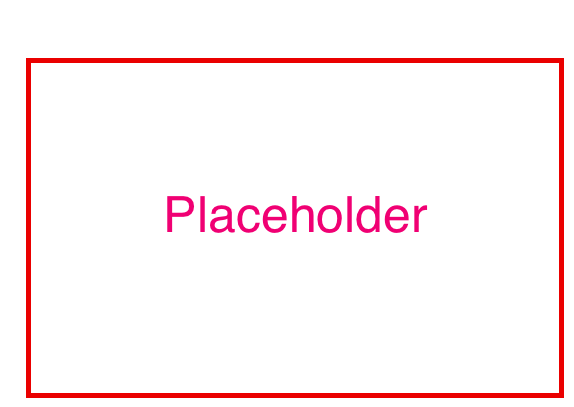
\includegraphics[width=0.6\textwidth]{Figures/placeholder.png}
  \label{fig:placeholder}
\end{figure}
% Mockups Upvote/downvote.

\item
\textbf{Favor Question}: If the student consider the question as a helpful and useful content and want to review this question in the future, he can favor the question and locate it in a certain list.

\begin{figure}[!htbp]
  \caption{placeholder}
  \centering
    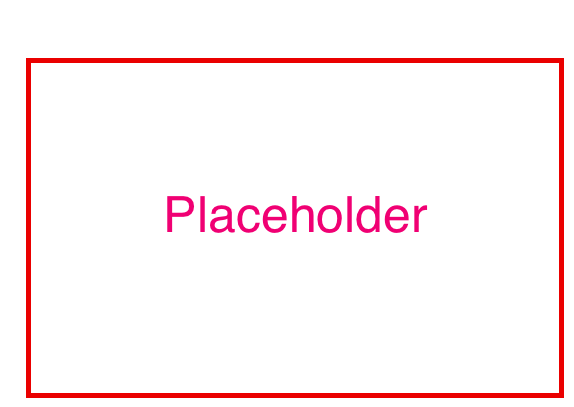
\includegraphics[width=0.6\textwidth]{Figures/placeholder.png}
  \label{fig:placeholder}
\end{figure}
% Mockups Fav, fav list

\item
\textbf{Accept Answer}: The owner of the question has the right to accept the most useful answer in his opion which will be shown up at the top of the answer list.

\begin{figure}[!htbp]
  \caption{placeholder}
  \centering
    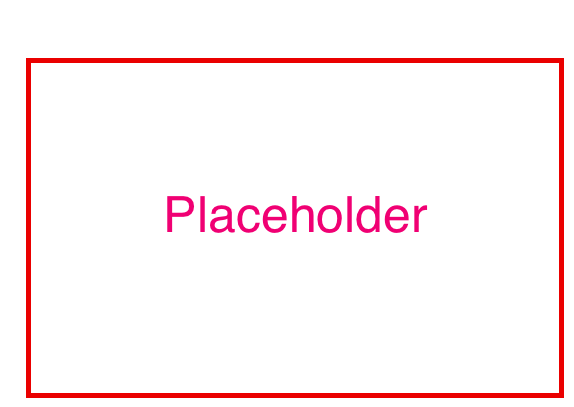
\includegraphics[width=0.6\textwidth]{Figures/placeholder.png}
  \label{fig:placeholder}
\end{figure}
% Mockups Accept, Top.

\end{enumerate}

\subsubsection{Answer Management}

\begin{enumerate}
\item
\textbf{Submit/Modify/Remove Answer}: User who has experence with the question can submit his answer to the question. After the submission, the modification or removal of the user's own question is possible.

\begin{figure}[!htbp]
  \caption{placeholder}
  \centering
    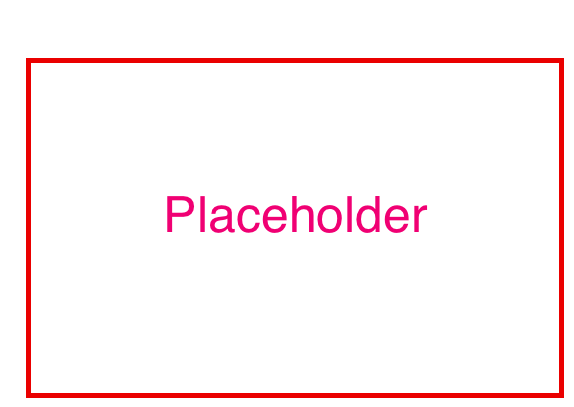
\includegraphics[width=0.6\textwidth]{Figures/placeholder.png}
  \label{fig:placeholder}
\end{figure}
% Mockups submit, withdraw

\item
\textbf{Upvote/Downvote Answer}: As mentioned above in section of question functionality, a similar idea of assessment should also be applied to answers. Answer with higher vote will be listed at first.

\begin{figure}[!htbp]
  \caption{placeholder}
  \centering
    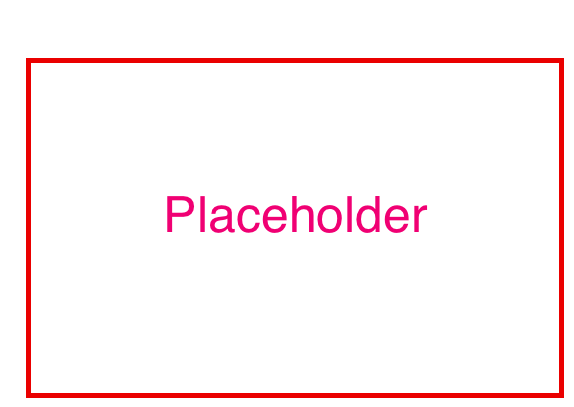
\includegraphics[width=0.6\textwidth]{Figures/placeholder.png}
  \label{fig:placeholder}
\end{figure}
% Mockups Upvote/downvote, arrange of answer.

\item
\textbf{Quote Answer}: Answers are able to be quoted so that the user can supplement informations on the top of original post or point out the deficiency of the contribute.

\begin{figure}[!htbp]
  \caption{placeholder}
  \centering
    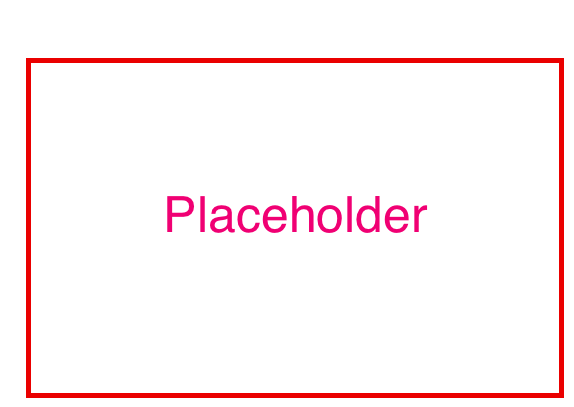
\includegraphics[width=0.6\textwidth]{Figures/placeholder.png}
  \label{fig:placeholder}
\end{figure}
% Mockups Fav, fav list

\end{enumerate}


\subsection{High Interativity}
Building with the basic functionalities is far not enough. To fit the system for educational purpose and improve the interactivity for arousing enthusiasm of students, a drawing tool and realtime functionality should be intergrated into the system.

\subsubsection{Drawing Tool}
Normally, some of the thoughts can't be simply expressed by textual description, so a drawing tool should be designed to enables the user to compose not only text but also different components such like rectangle, circle, line and so on, which helps the user to express his question more precisely.
The ideal drawing tool should have following features:

\begin{enumerate}
\item
\textbf{Drawing Diverse Components}: Not only text but also diverse components could be drawn while posting a contribution. Styling of a component such as size tuning, color changing is also the essential, which will helps emphasize the important part the user expressing.

\begin{figure}[!htbp]
  \caption{placeholder}
  \centering
    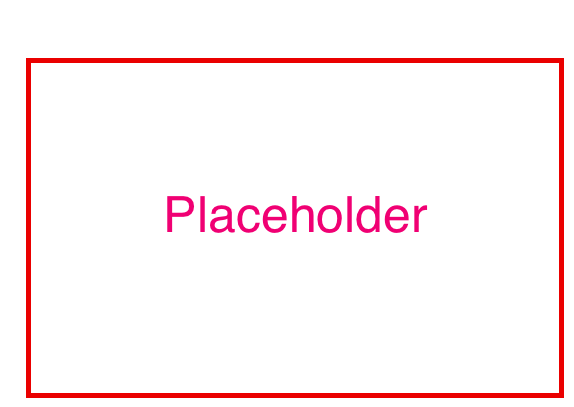
\includegraphics[width=0.6\textwidth]{Figures/placeholder.png}
  \label{fig:placeholder}
\end{figure}
% Mockups draw components, styling

\item
\textbf{Drawing History}: During drawing, the user might make mistakes or change mind after placing a component or text. So a history list of drawing actions bundled with undo and redo functionalities will dramatically improve the usability of drawing process.

\begin{figure}[!htbp]
  \caption{placeholder}
  \centering
    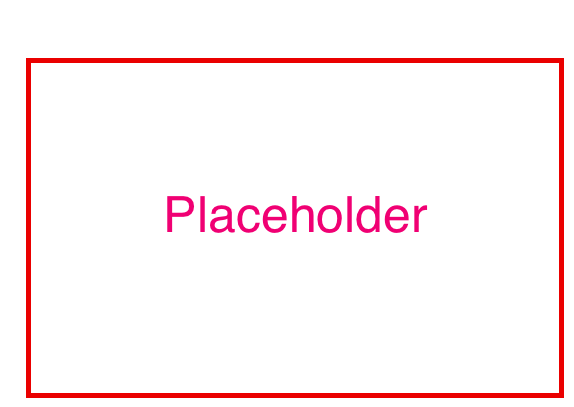
\includegraphics[width=0.6\textwidth]{Figures/placeholder.png}
  \label{fig:placeholder}
\end{figure}
% Mockups history list, undo, redo


\end{enumerate}


\subsubsection{Realtime}
How to ease the approach of content acquisition and improve the interactivity for arousing enthusiasm of students, is also a key point while designing the discuss system. So two major realtime functionalities are featured as follow: 

% Auto Ordering of Questions / Answers
% Sidebar notifications!

\begin{enumerate}
\item
\textbf{Realtime Question List}: Without requesting the question list initiatively, all new questions posted by other users will be pushed to user automatically. The user doesn't have to concern himself with acquisition of the new content anymore.

\begin{figure}[!htbp]
  \caption{placeholder}
  \centering
    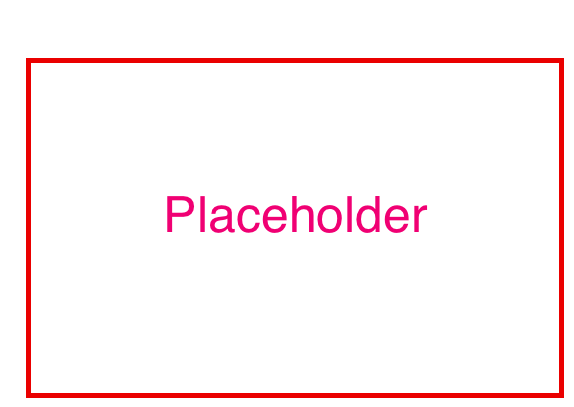
\includegraphics[width=0.6\textwidth]{Figures/placeholder.png}
  \label{fig:placeholder}
\end{figure}
% Mockups submit, withdraw

\item
\textbf{Realtime Answer Ordering}: Without refreshing the page, the answers will be re-ordered as new vote action is triggered.

\begin{figure}[!htbp]
  \centering
    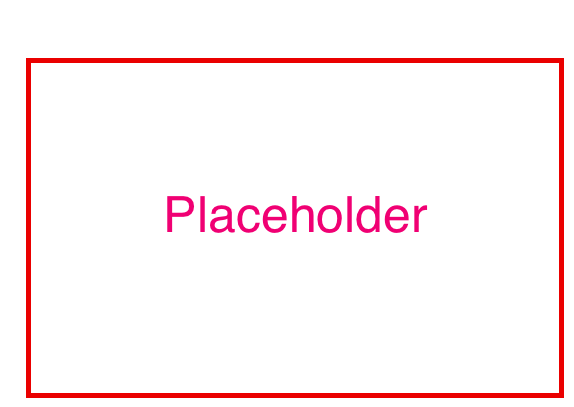
\includegraphics[width=0.6\textwidth]{Figures/placeholder.png}
  \label{fig:placeholder}
  \caption{placeholder}
\end{figure}
% Mockups Upvote/downvote, arrange of answer.


\end{enumerate}
